\chapter{Related software}

There are plenty of programs and libraries for graph visualization with different purposes.
Just to name a few there are D3.js, Neo4j, Graphviz, Tulip, Wolfram Grapher, Pajek and many more.

In this chapter however I'm going to focus on just three software products - each with very different use-case and target userbase.

\begin{itemize}

\item The first one is \textbf{Obsidian} which is primarily a note-taking application
but provides a graph view of the notes as an interesting and easy to use feature. 

\item The second is \textbf{Gephi}, a software focused on in-depth analysis and visualization of large graphs.

\item And finally there's \textbf{Cytoscape.js}. A javascript library for graph visualization in the browser.

\end{itemize}

I chose these in particular because Afantázie could be viewed as a hybrid of the trio.

We will look into three aspects of these products:
\begin{itemize}
  \item Primary use-case and target userbase
  \item User experience
  \item Ability to visualize large graphs
\end{itemize}

As the source of data for testing the large-graph visualization capabilities I chose the dataset of citations between papers
in the field of high-energy physics \xxx{(CitHep) \cite{snap_cit_hep}} (Later refered to as the CitHep dataset).
It contains 34546 nodes, 421578 edges and temporal data.

This dataset is suitable for my purposes because:
\begin{itemize}
  \item It's large enough to test the the capabilities of both the mentioned software and Afantázie
  \item It's a real-world dataset with temporal data which is going to play a role in visualizing the contents of Afantázie
\end{itemize}

\section{Obsidian}

Obsidian was a direct inspiration for Afantázie. It allows users to create, edit and most importantly interlink markdown file notes in the file system.
One Obsidian project is just a system directory called a Vault. It is a set of markdown notes, user settings, plugins and other files.
The interlinked notes in a Vault form a directed graph which can be visualized with just a click of a button.
The graph is animated and has the ability to replay the history of the Vault from the very first note to the current state.

It's clear from this description that Obsidian is aimed at general audience of note-takers 
with maybe a slight bias towards graph/data visualization enthisuiasts.
It's available for all the major operating systems and has a large community of users and plethera of extensions available through the
community plugins.

\subsection{Obsidian graph view}

The graph visualization in obsidian (called graph view) is based on a force-directed layout algorithm \xxx{(more in chapter TBD)}.
It is easy to use and provides an appealing visual representation of the notes. It is also customizable to some extent.

Colors of the nodes can be set based on different filters such as path, tags or text-search.
Users can also adjust four sliders - central force, repel force, link force and link distance.
The graph view is sufficient for small graphs but for larger graphs the program needs to spend some time indexing the notes.
(Though, this is a one-time operation and the indexes are then saved in the Vault).

In figure \ref{obr:obsidian_common} you can see a typical Obsidian graph view depicting a small Vault of one of my personal projects.

In figure \ref{obr:obsidian_3000} I converted a part of the CitHep dataset with only the first 3000 nodes to markdown notes and visualized it in Obsidian.
It took my machine over 10 minutes to index this graph and I was unable to visualize the whole dataset without the program crashing or taking too long to index.
Once indexed however the application ran smoothly.

Obsidian is not very good at clustering nodes with high degree of connectivity.
To my knowledge it also has no support for automatic colouring of the nodes based on clusters, modularity  or other data indicators.
Color has to be user defined which is why the graph in figure \ref{obr:obsidian_3000} is all default gray.

\xxx{TODO - proportions of the image(s)}
\begin{figure}[p]\centering
  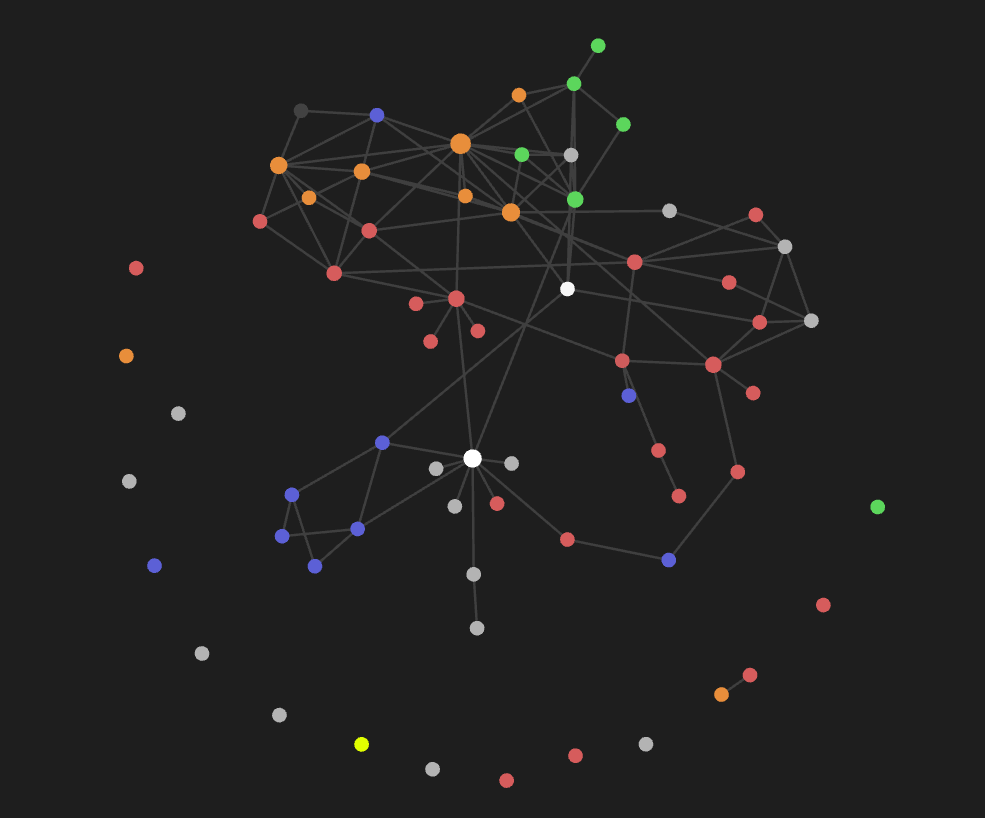
\includegraphics[width=140mm, height=140mm]{img/obsidian_common_notes.png}
  \caption{A common graph view of a small Vault in Obsidian}
  \label{obr:obsidian_common}
\end{figure}


\begin{figure}[p]\centering
  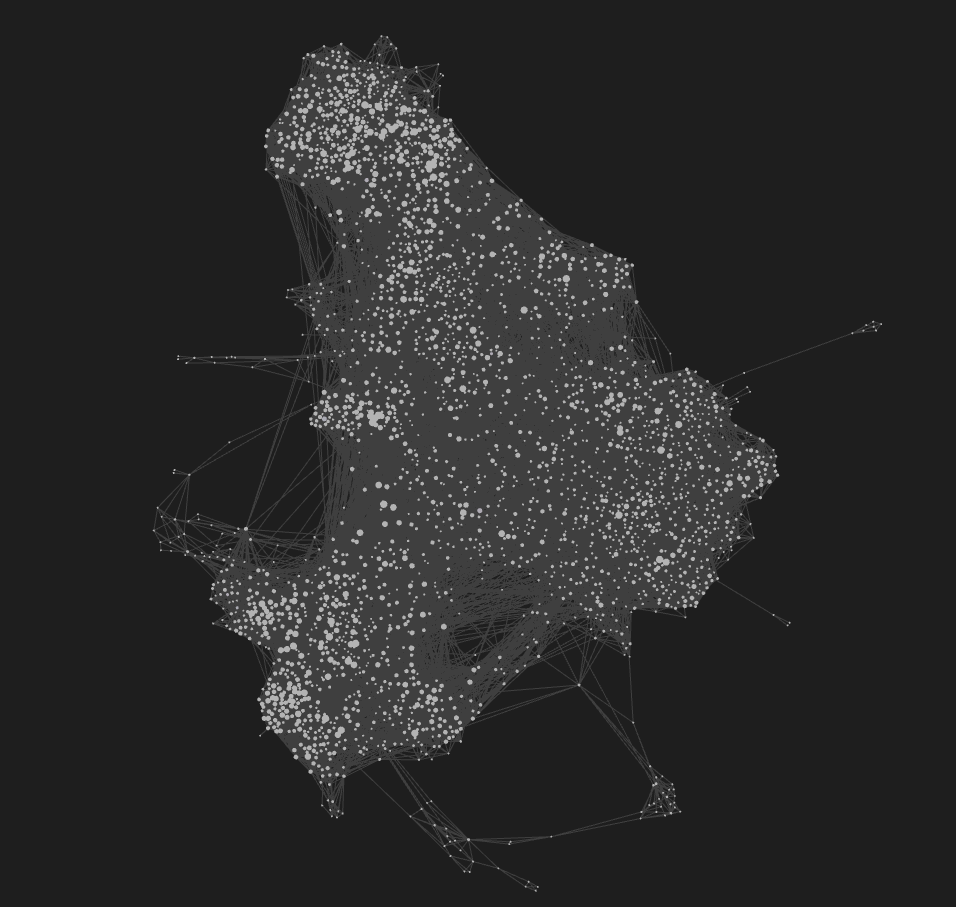
\includegraphics[width=140mm, height=140mm]{img/Obsidian_3000}
  \caption{The first 3000 nodes of the CitHep dataset visualized in Obsidian}
  \label{obr:obsidian_3000}
\end{figure}

\section{Gephi}

Much more specialized than Obsidian, Gephi is an open source software focused on visualization and quantitative analysis of large graphs.
It provides tens and with plugins hundreds \xxx{(cit. needed)} algorithms for graph layout and quantitative analysis of various data.

Gephi can compute quantitative characteristics of graph-based data such as modularity, clustering coefficient, degree distribution and many more.
It can not just vizualize the working data in the viewport but also export rather visually appealing images of the vizualized graph.

\subsection{Gephi graph export}

In figure \ref{obr:gephi_cithep_3k} you can see, again, the first 3000 nodes of the CitHep dataset visualized in Gephi.
Compared with Obsidian the Gephi redner provides more visually identifiable characteristics of the data:

\begin{itemize}
  \item The layout is more structured and communities are more visible
  \item Colors of the nodes represent their associated modularity class
  \item Size of the nodes represents the number of citations the associated paper has (or in-degree)
\end{itemize}

Figure \ref{obr:gephi_cithep} is an exported image of the entire CitHep dataset visualized in Gephi.
The process of exporting this image took a few hours.
I had to learn to use the program itself, import the data,
tweak the layout using various provided algorithms (though I mostly relied on ForceAtlas 2) and finally I exported the resulting image.

The software crashed a few times during the process and with the citHep dataset loaded in memory wasn't awlays buttery smooth but it was otherwise very usable.
Considering the amount of data that's a commendable feat.

% Online you can find even larger datasets visualized using Gephi. This one \link{https://forum-gephi.org/viewtopic.php?f=28&t=2314} for example consists of 212 600 nodes and 4 045 203 edges.

The user experience of Gephi is one of a technical tool - something you have to learn to use and spend time with to get the most out of.
But the reward is the ability to visualize and analyze large graphs better than with any other software I could find.

\begin{figure}[p]\centering
  \includegraphics[width=140mm, height=140mm]{img/gephi_first_3000.png}
  \caption{The first 3000 nodes of the CitHep dataset visualized in Gephi}
  \label{obr:gephi_cithep_3k}
\end{figure}


\begin{figure}[p]\centering
  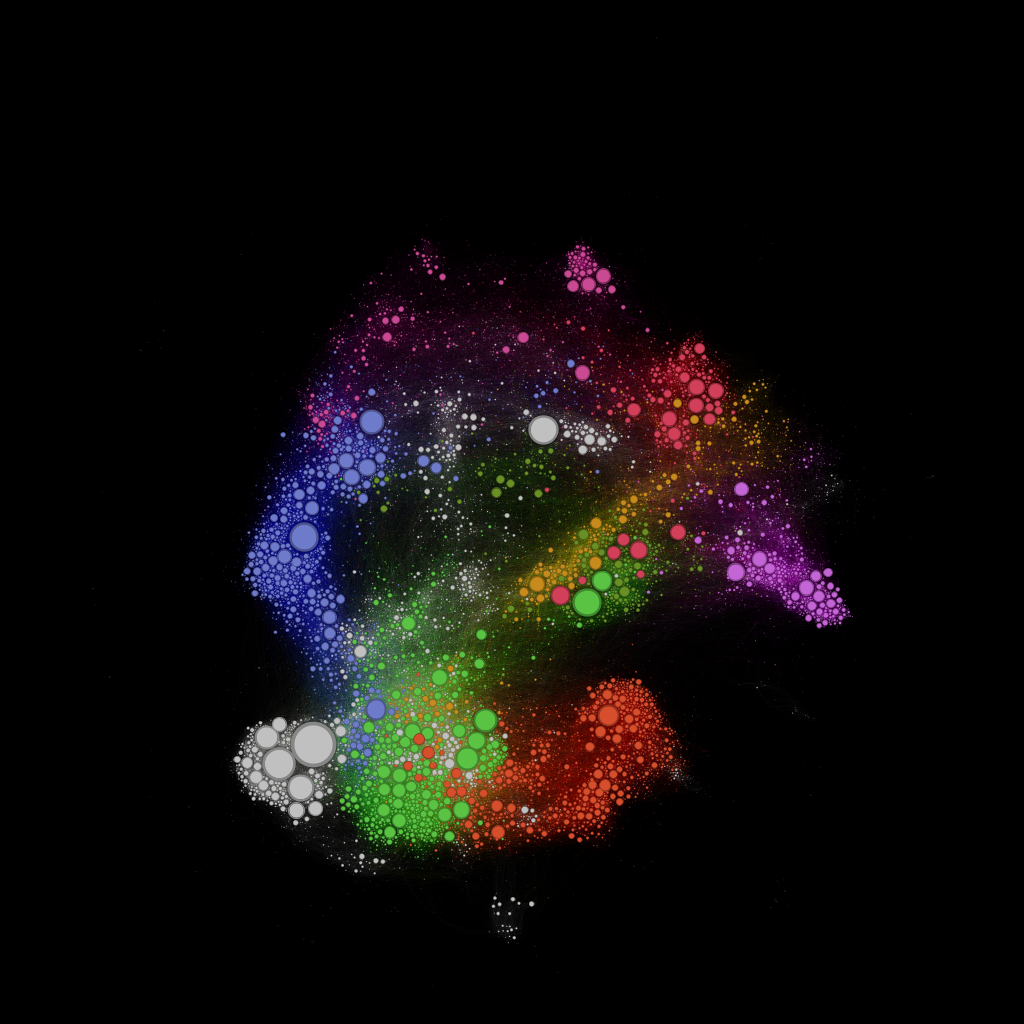
\includegraphics[width=140mm, height=140mm]{img/gephi_cithep_35k.png}
  \caption{CitHep dataset visualized in Gephi (34546 nodes)}
  \label{obr:gephi_cithep}
\end{figure}

\section{Cytoscape.js}
Cytoscape.js is a javascript library for graph visualization in the browser.
\xxx{TODO - Vyzkoušet}

\section{Final comparison}